\documentclass[12pt, twoside, openany]{report}
\usepackage[dvips]{graphicx,color,rotating}
\usepackage[cp1250]{inputenc}
\usepackage{t1enc}
\usepackage{a4wide}
\usepackage{amsfonts}
\usepackage{amsmath}
\usepackage{enumerate}
\usepackage{verbatim}
\usepackage[MeX]{polski}
\usepackage[T1]{fontenc}
\usepackage{geometry}
\geometry{left=25mm,right=25mm,%
bindingoffset=10mm, top=25mm, bottom=25mm}
\usepackage{amssymb, latexsym}
\usepackage{amsthm}
\usepackage{palatino}
\usepackage{array}
\usepackage{pstricks}
\usepackage{textcomp}
\theoremstyle{definition}
\newtheorem{theorem}{Twierdzenie}[section]
\newtheorem{remark}{Uwaga}[section]
\newtheorem{definition}{Definicja}[section]
\newtheorem{alg}{Algorytm}[chapter]
\newtheorem{prz}{Przypadek}[section]
\newtheorem{np}{Przyk�ad}[section]
\newtheorem{lemma}[theorem]{Lemat}
\linespread{1.5}
\newcommand*{\norm}[1]{\left\Vert{#1}\right\Vert}
\newcommand*{\abs}[1]{\left\vert{#1}\right\vert}
\newcommand*{\om}{\omega}

\author{Autor}
\title{Tytu� pracy}

\begin{document}

% Za��� g�l� ja��.
\begin{titlepage}
\pagestyle{empty}

\noindent
\begin{Large}
\begin{table}[t]
\centering
\begin{tabular}[t]{lcr}

& WYDZIA� IN�YNIERII & \\
& BIOMEDYCZNEJ &
\end{tabular}
\end{table}

% \vfill
\begin{center}PROJEKT\end{center}
\begin{center}BIOCYBERNETYKA\end{center}\end{Large}
% \vfill
\begin{center}
\Huge
\textbf{Automaty kom�rkowe}

\end{center}
% \vfill\vfill
\begin{center}

\includegraphics[scale=0.8]{logo}

\end{center}

\vfill
\begin{center}
\normalsize
Autorzy:\\
\Large
D�esika Szyma�ska, Oliwia Drozdek, Marlena Mruczek
\end{center}

\begin{center}
\large
Zabrze, stycze� 2018
\end{center}




% \maketitle
\end{titlepage}
\tableofcontents
\thispagestyle{empty}
\newpage
\pagestyle{headings}
\setcounter{page}{1}


%-----------Pocz�tek cz�ci zasadniczej-----------

\chapter{Cel pracy}
Celem projektu jest przedstawienie tematu automat�w kom�rkowych - pozyskanie wiedzy na temat ich dzia�ania oraz zastosowania. Efektem realizacji jest zaprojektowanie aplikacji z interfejsem graficznym.

\chapter{Wprowadzenie}

\chapter{Opracowanie teoretyczne}

\chapter{Specyfikacja wewn�trzna}

Do stworzenia aplikacji zosta�o wykorzystane �rodowisko app designer w matlabie. 
Aplikacja zawiera 4 regu�y � ka�da z nich posiada w�asn� metod�. Metody te przyjmuj� parametr app, kt�ry pozwala na korzystanie z pozosta�ych komponent�w programu. W ciele funkcji zostaje modyfikowana siatka GRID w niesko�czonej funkcji for. Modyfikacja zale�y od zadanych warunk�w, kt�re s� specyficzne dla konkretnej regu�y. Wynik jest prezentowany graficznie � przedstawienie siatki GRID.

\chapter{Specyfikacja zewn�trzna}

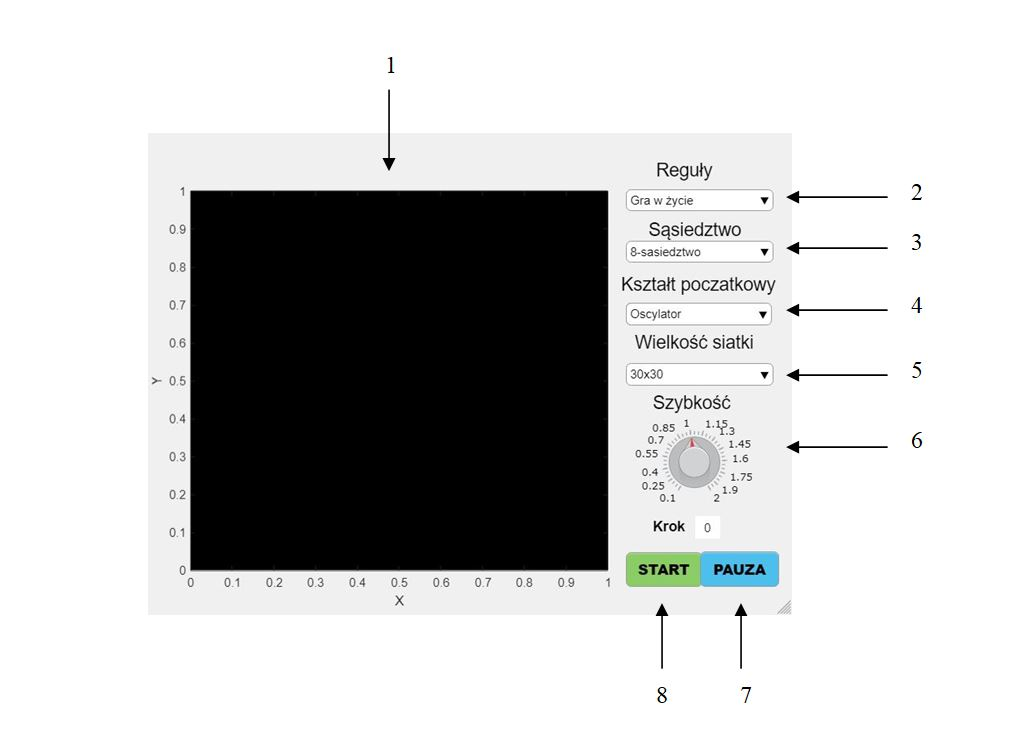
\includegraphics[scale=0.6]{zd}





\chapter{Wyniki}
\chapter{Podsumowanie}


%-----------Koniec cz�ci zasadniczej-----------

\begin{thebibliography}{11}
\bibitem[1]{B} Stanis�aw Bia�as, \emph{Macierze. Wybrane problemy}, AGH Uczelniane Wydawnictwa Naukowo-Dydaktyczne, Krak�w, 2006.
\bibitem[2]{H} Nicholas J. Higham, \emph{Accuracy and stability of numerical algorithms}, SIAM, Philadelphia 1996.
\bibitem[3]{H2} Nicholas J. Higham, \emph{Functions of Matrices. Theory and Computation}, SIAM, Philadelphia 2008.
\bibitem[4]{DJ} Maksymilian Dryja, Janina i Micha� Jankowscy, \emph{Przegl�d metod i algorytm�w numerycznych, cz�� 2}, Wydawnictwa Naukowo-Techiczne, Warszawa 1982.
\end{thebibliography}


\end{document}